\section*{External delay optimization}

\section*{Time resolution behaviour as a function of energy}
In order to study the time resolution dependence as a function of the energy we have used a different radioacive source, $^{60}$Co. This source is chosen because of its high energy Compton Edge (1 MeV) that allow us to study the energy dependence up to this energy. 

\smallskip

\noindent By imposing a lower energy threshold starting from 100 keV to 1000 keV we are able to plot the time resolution as a function of the lower energy threshold (Fig.\ref{Fig: lower energy thr}~).

\smallskip

\begin{figure}[h!]
\centering
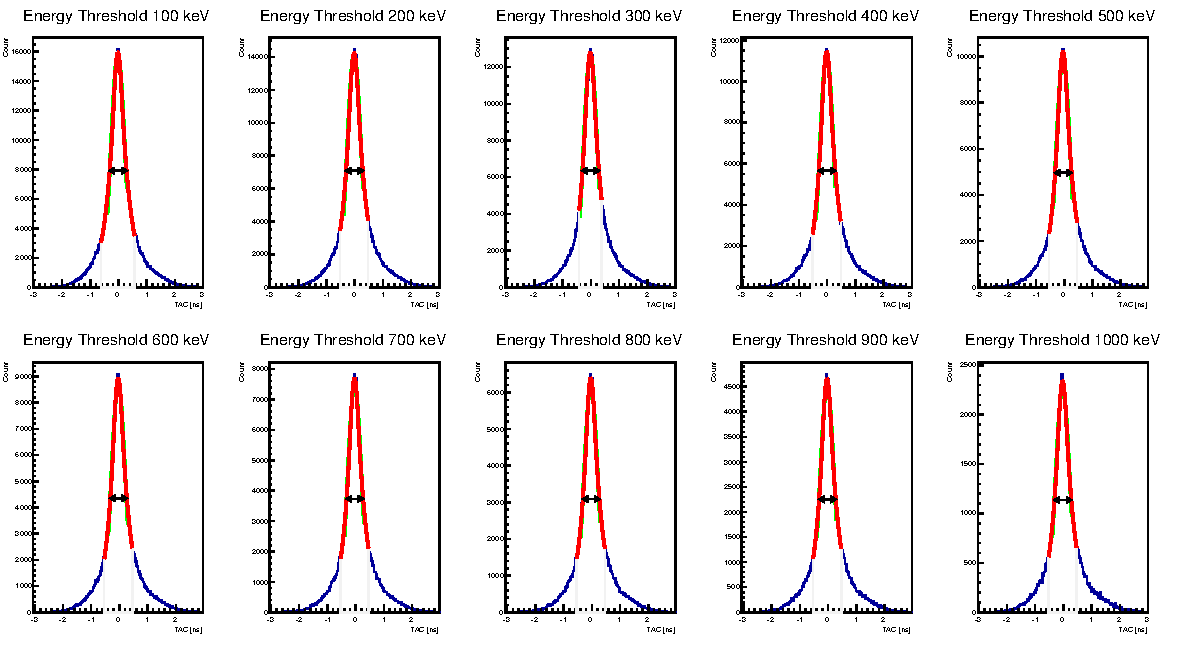
\includegraphics[width = \textwidth]{ThresholdTAC_dists}
\caption{Timing distributions using threshold.}
\label{Fig: lower energy thr}
\end{figure}

\begin{figure}[h!]
\centering
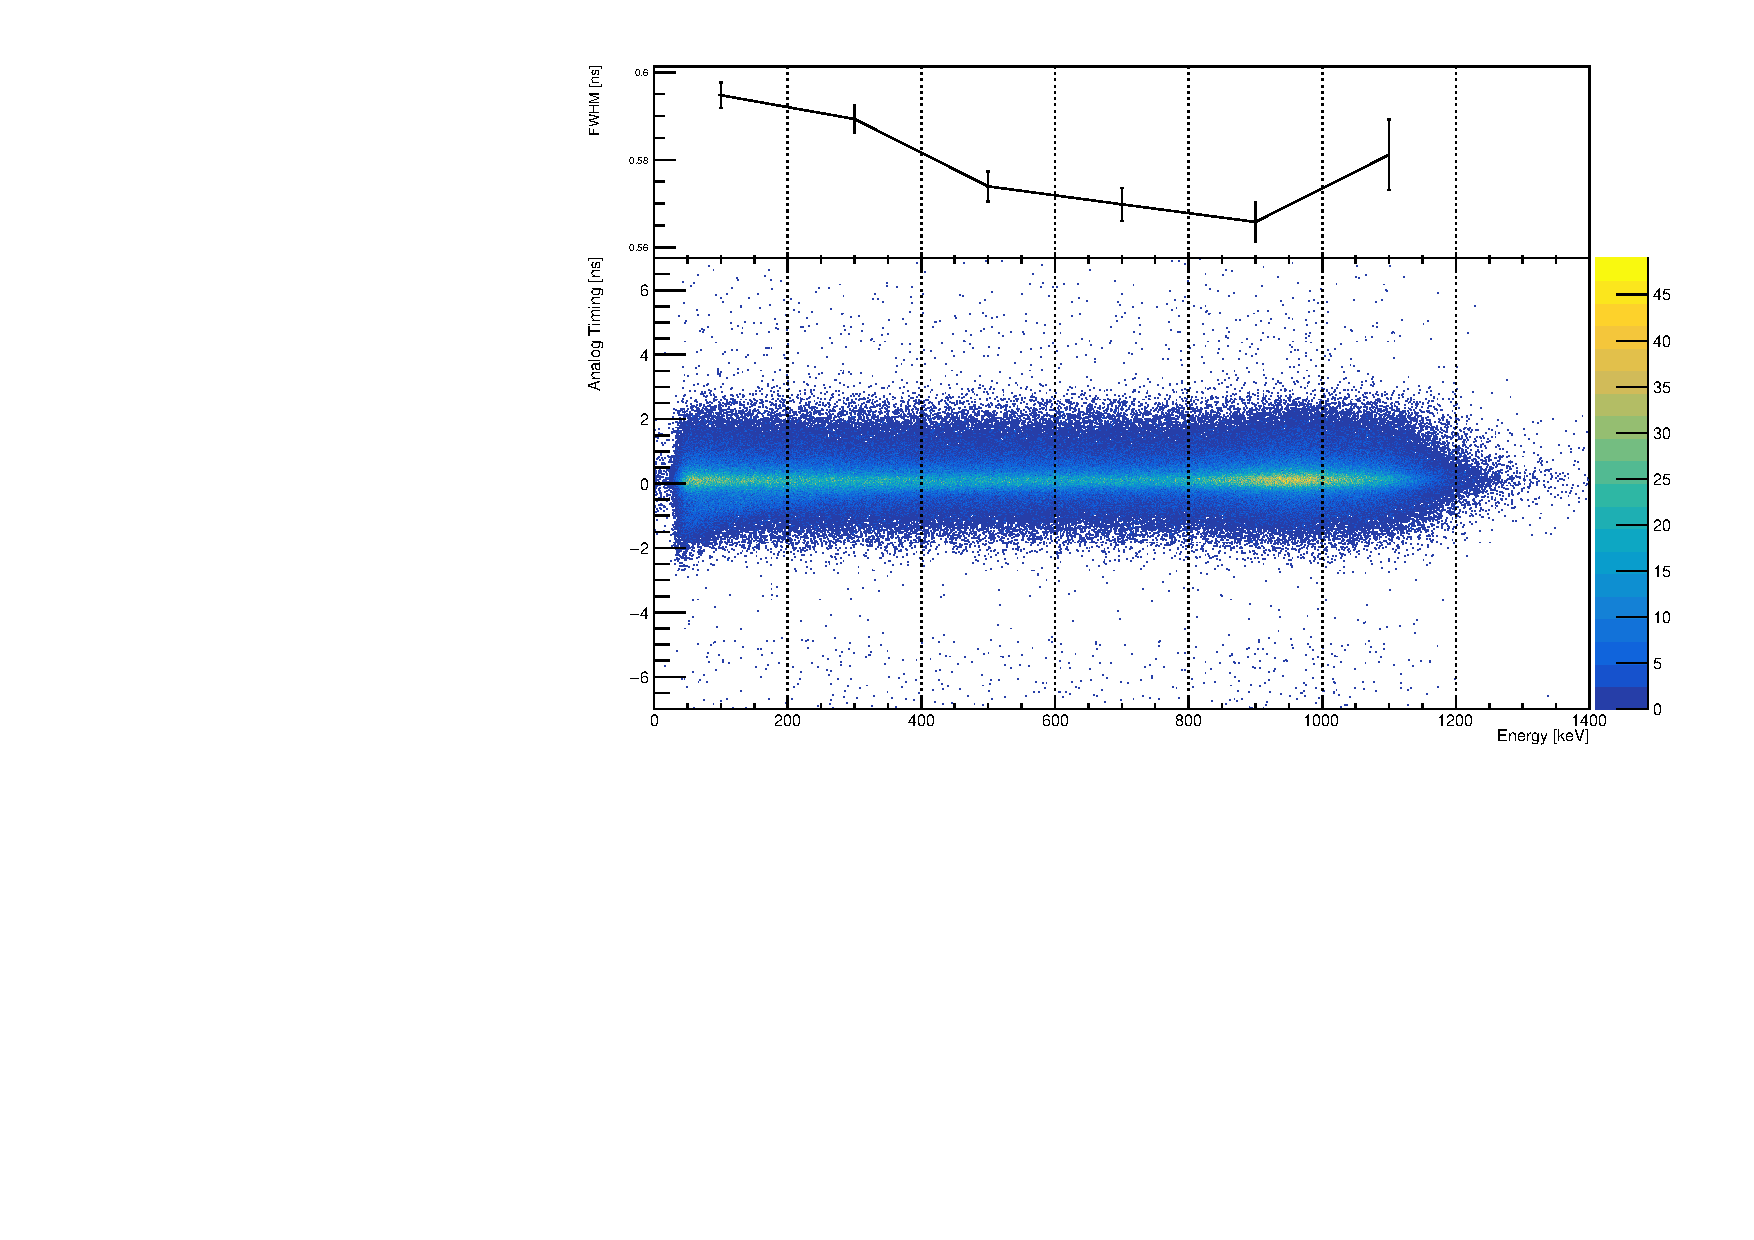
\includegraphics[width = 1\textwidth]{ThresholdTAC_FWHMvs2Ddist}
\caption{Lower energy threshold.}
\label{Fig: lower energy thr}
\end{figure}


\smallskip

\noindent We can also proceed in a slightly different way: instead of setting a lower energy threshold we can select energy windows with 100 keV of width and plotting the time resolution in function of the energ mid-energy (Fig. \ref{fig: energy windows analog}~).

\begin{figure}[h!]
\centering
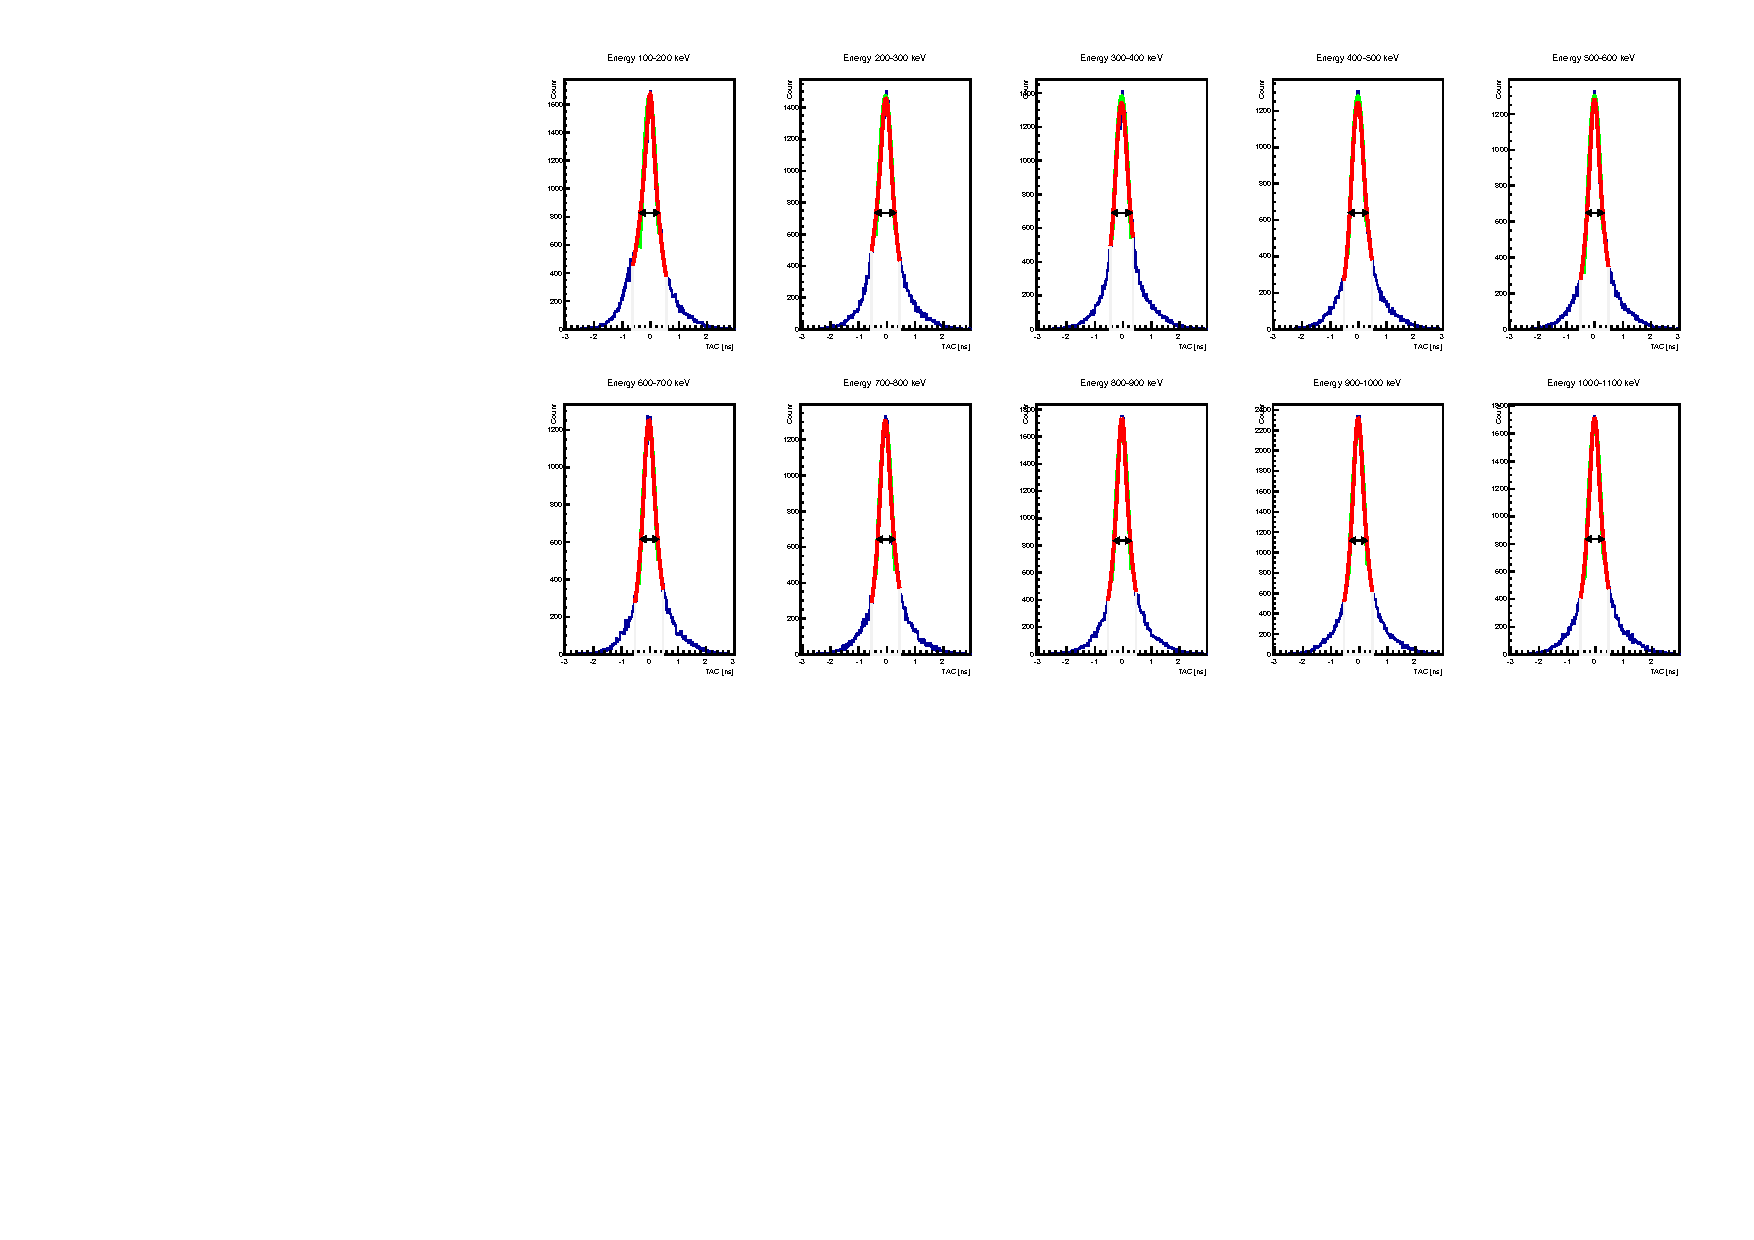
\includegraphics[width = \textwidth]{SlicedTACdists}
\caption{Timing distributions using threshold.}
\label{Fig: lower energy thr}
\end{figure}

\begin{figure}[h!]
\centering
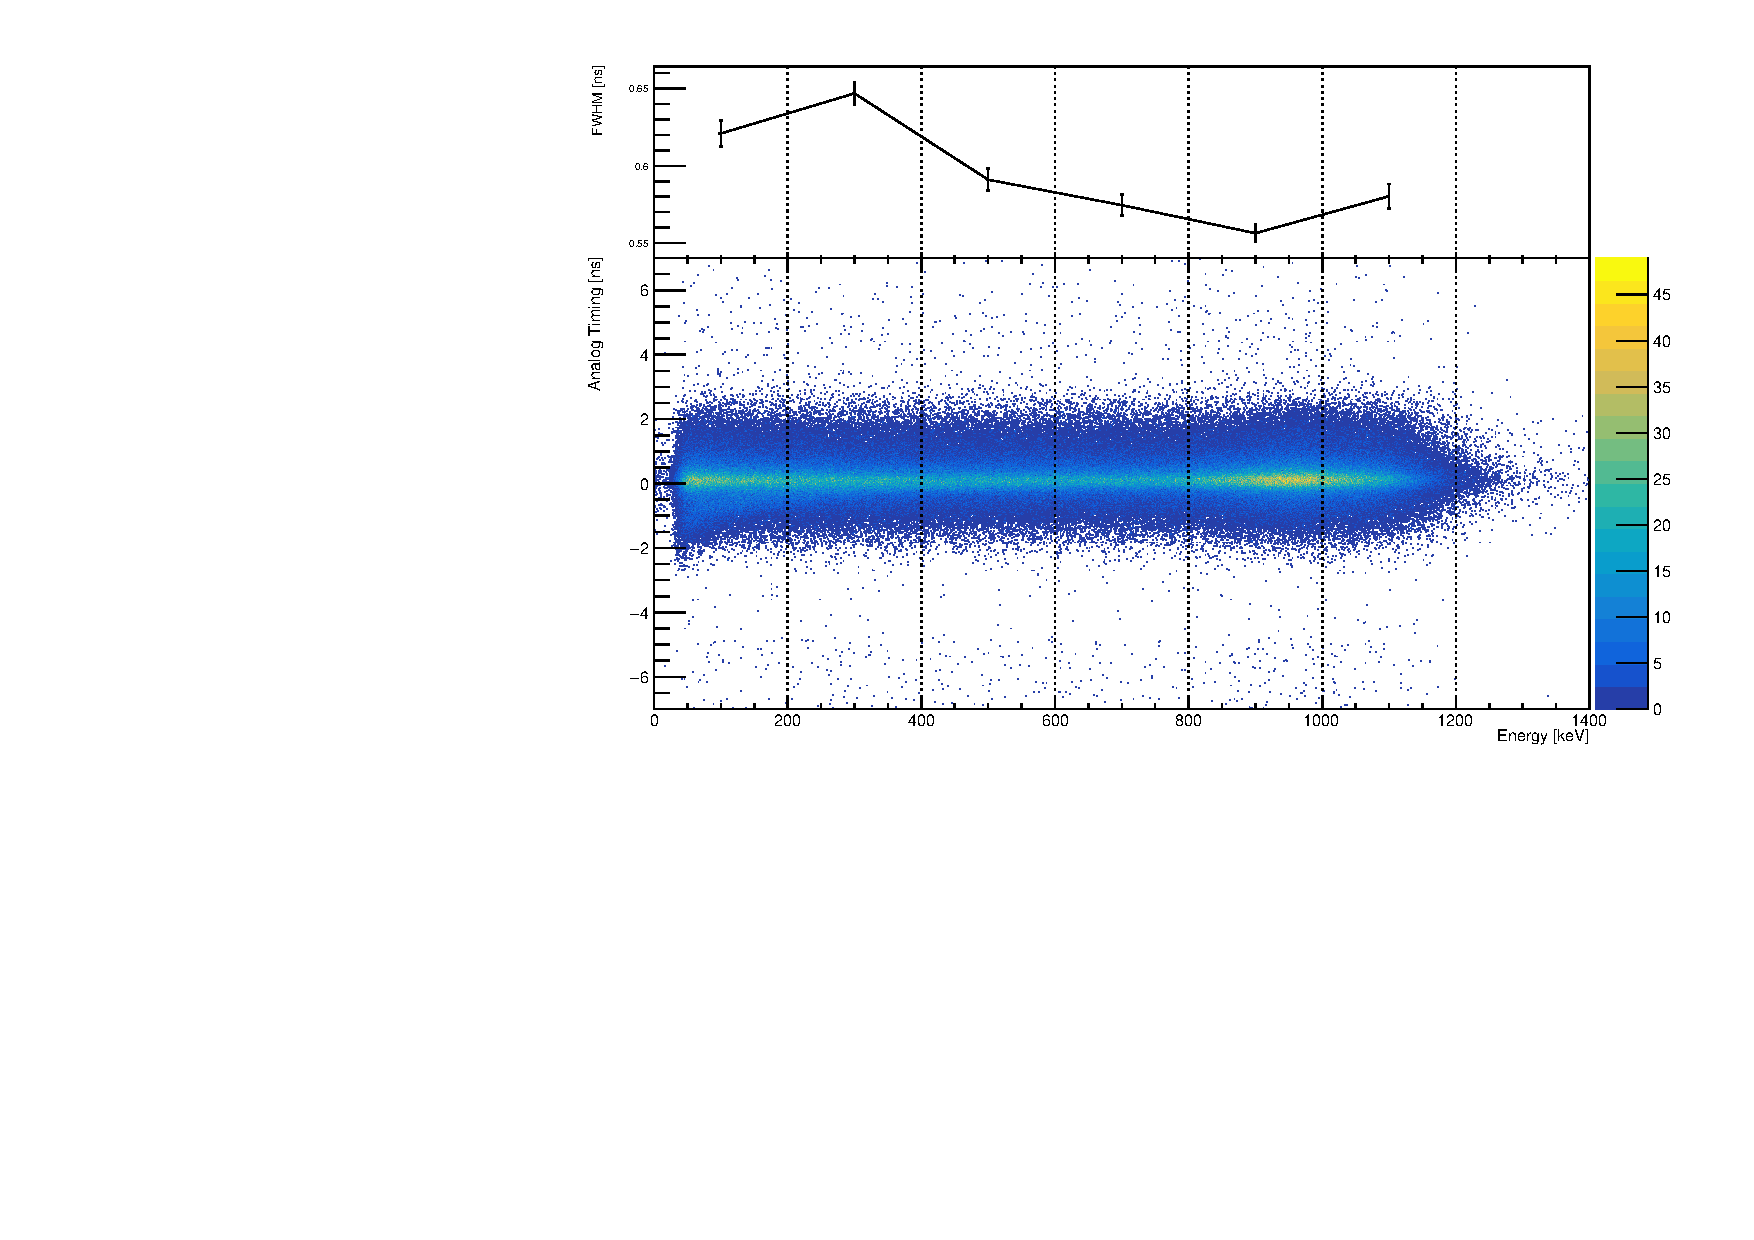
\includegraphics[width = \textwidth]{SlicedTAC_FWHMvs2Ddist}
\caption{Energy Windows}
\label{fig: energy windows analog}
\end{figure}

% Dobbiamo commentare i risultati dopo le misure e 
% scrivere qual è la differenza tra soglie e finestre
\noindent The time resolution behaviour obtained with these two different methods have the same shape but we can clearly see that the use of energy windows allow to determine the time resolution with a lower constant error due to the fact that we 






















